\documentclass[a4paper,12pt]{article}

%% Standard
\usepackage[ngerman]{babel} 
\usepackage[utf8]{inputenc}
\usepackage[T1]{fontenc}

%% Mathe
\usepackage{amsmath}
\usepackage{amssymb}
\usepackage{amsthm}
\usepackage{latexsym}

%% Aufzaehlungen
\usepackage{enumerate}

%% Bilder
\usepackage{subfigure}
\usepackage{graphicx}

%% Absaetze usw
\usepackage{multicol}   
% zu verwenden mit 
% \begin{multicols}{$$Spaltenanzahl$$} 
%  text...
% \end{multicols}

%\setlength{\parindent}{0pt}    %Absatz-Einrueckung
%\setlength{\parskip}{3pt}      %Absatz-Abstaende


%% Fusszeilen
\usepackage{fancyhdr}
\pagestyle{fancy}
\renewcommand{\headrulewidth}{0pt}
\renewcommand{\footrulewidth}{0.4pt}
\lfoot{\NAME : \TITEL}
\cfoot{}
\rfoot{\thepage}
\lhead{}
\chead{}
\rhead{}
%\setlength{\headheight}{15pt}


%% Links
\usepackage[colorlinks=true,linkcolor=black,citecolor=black,%
bookmarksnumbered=true,breaklinks=true,pdfstartview=FitH]{hyperref}

%% Eigene Kommandos
% Differenzialrechnung
\newcommand{\diff}{\ensuremath{\mathrm d}}
\newcommand{\dx}{\ensuremath{\mathrm dx}}
\newcommand{\dvx}{\ensuremath{\mathrm d \vec x}}

% Lineares
\newcommand{\Mat}[1]{\ensuremath{\mathbf{#1}}}
\newcommand{\Ten}[1]{\ensuremath{\mathcal{#1}}}
\newcommand{\Ve}[1]{\ensuremath{\vec{#1}}}
% Vektoren sind Fette buchstaben
\renewcommand{\vec}[1]{\ensuremath{\boldsymbol{#1}}}
% Vektoren sind fett und nicht kursiv
% \renewcommand{\vec}[1]{\ensuremath{\mathbf{#1}}}
\newcommand{\skp}[2]{\ensuremath{\langle #1 \,|\, #2 \, \rangle}}


% Euler
\newcommand{\e}{\ensuremath{\operatorname{e}}}
\newcommand{\E}{\ensuremath{\operatorname{e}}}
\newcommand{\ir}{\ensuremath{\operatorname{i}}}
\newcommand{\I}{\ensuremath{\operatorname{i}}}

% allg Mathe
\newcommand{\R}{\ensuremath{\mathbb{R}}}
\newcommand{\folgt}{\ensuremath{\Rightarrow}}
\newcommand{\gdw}{\ensuremath{\Leftrightarrow}}


% Formatierung
\newcommand{\abs}[0]{\bigskip\noindent}
\newcommand{\const}{\ensuremath{\text{\emph{const}}}}


% Umgebungen
\newtheorem{satz}{Satz}[section]
\newtheorem{defi}{Definition}[section]
\newtheorem{lemma}{Lemma}[section]






\begin{document}



\newcommand{\NAME}{Michael Kopp}
\newcommand{\FACH}{Physik am Komputer}
\newcommand{\TITEL}{"Ubung 03}
\newcommand{\DATUM}{\today}


\pagestyle{plain} 
	% auskommentieren fuer fusszeile



%%%% Eigener Kopf

\sloppy

\begin{center}
\FACH
\hfill
\DATUM
\end{center}

\vspace{-5mm} % weniger abstand

\begin{center}
  \begin{Large}
 \textbf{\TITEL}
  \end{Large}
\end{center}

\vspace{-3mm}

\begin{center}
\hrulefill
%\quad
 %\raisebox{-1.5mm}{\NAME}
% \,
\quad 
\textit{\NAME}
\,
\hrulefill
\end{center}
 
 
%%%%%%%%%%%%%%%%%%%%%%%%%%%%%
%%%%%%%%%%%%%%%%%%%%%%%%%%%%%%
%%%%%%%%%%%%%%%%%%%%%%%%%%%%%%%%


\paragraph{Aufgabe 1}

Ich habe -- wie in der "Ubung besprochen -- nur den letzten Punkt gemacht, weil
die Aufgabenstelltung der ersten Punkte nicht ganz verst"andlich war und wohl
dem "Ubungseffekt gedient hat, um auf den letzten Punkt hinzuarbeiten\dots

Die Bem"uhungen hierzu gipfelten in \texttt{fibon-rekt01c.cpp}.




\paragraph{Aufgabe 2}

Die ersten beiden Punkte wurden in \texttt{numdiff03.cpp} sogar "ubertroffen:
Ich habe noch die Ableitung einer Ordnung h"oher eingef"ugt. Die Bem"uhungen
sind in Abb. \ref{fig:vgl-abl} am besten visualisiert (alle Graphiken finden sich in
\texttt{abl-*.eps}).


\begin{figure}[h]
	\begin{center}
		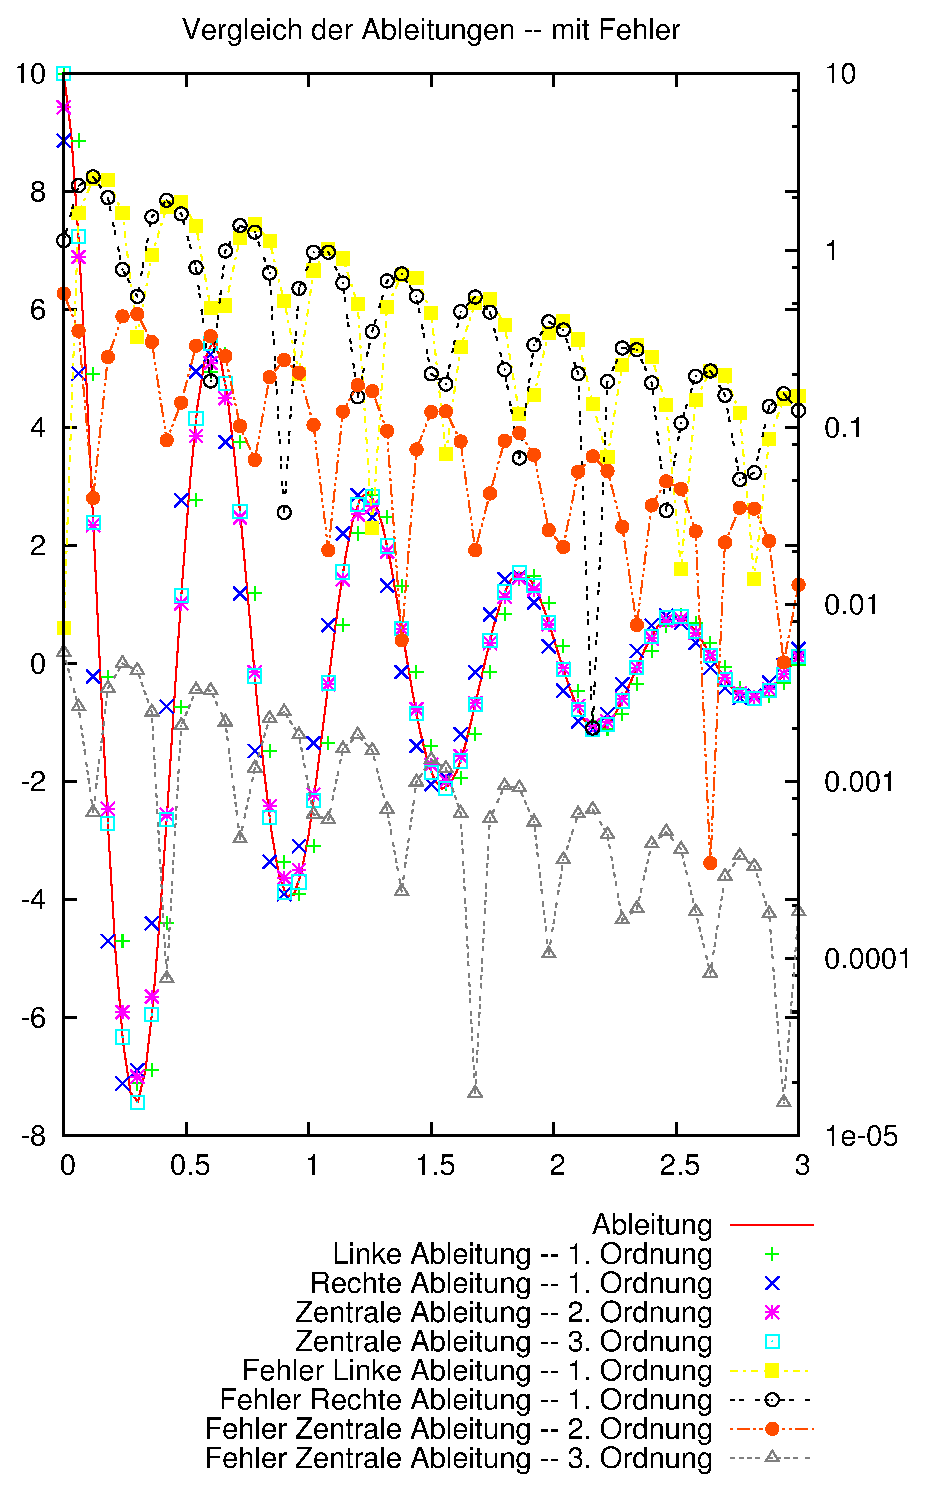
\includegraphics[width=\textwidth]{./vgl-abl.eps}
	\end{center}
	\caption{Vergleich der Ableitungen verschiedener Ordunungen}
	\label{fig:vgl-abl}
\end{figure}


\abs
Zum dritten Punkt:

Approximiere die Funktino an den St"utzstellen $x_1, \dots, x_5$ durch ein Polynom der vierten Ordnung; am besten geht das mit Lagrange-Polynomen:
\begin{equation}
	p_4(x) = \sum_{i=1}^{5} \prod_{j = 1, j \neq i}^5 f(x_i) \cdot \frac{x-x_j}{x_i-x_j} \;.
	\label{eq:p4}
\end{equation}
Leitet man dies an der Stelle $x_3$ ab und setzt "aquidistante St"utzstellen ein (also $x_1 = x_3 - 2h$, $x_2 = x_3-h$ usw), dann erh"alt man die Gleichung
\begin{equation}
	-{{ y_{5}-8\,y_{4}+8\,y_{2}-y_{1}}\over{12\,h}} \;;
	\label{eq:ablnaehr}
\end{equation}
vergleiche zur Rechnung \texttt{numdiff\_ord4}.

Nun entwickelt man die Funktion $f(x)$ um $x$ und zwar f"ur $y_5$ in Richtung $x + 2*h$, f"ur $y_2$ in Richtung $x - h$ etc. und setzt die so erhaltenen Entwicklungen in \ref{eq:ablnaehr} ein; es ergibt sich (f"ur die Rechnung vergleiche \texttt{numdiff\_ord4\_enwt})
\begin{equation}
	{ {h^4\,{\it y_5}-30\,{\it y_1}}\over{30}} = f'(x) + O(h^4) \;.
	\label{eq:ordn}
\end{equation}
\qed


\paragraph{Aufgabe 3}

Die Implementierungen sind in \texttt{numint03.cpp}, die Ergebnisse sind in
Abb. \ref{fig:vgl-int}
graphisch dargestellt. Man sieht: am langsamsten konvergiert das
Trapezverfahren, das Gaussverfahren der Ordnung 4 am schnellsten.

\begin{figure}[h]
	\begin{center}
		\includegraphics[width=\textwidth]{numint03}
	\end{center}
	\caption{Entwicklung der numerischen Integrationen $\int_0^3 \sin(10 x) \exp(-x)$ mit verschiedenen Verfahren}
	\label{fig:vgl-int}
\end{figure}




\end{document}














%%% Local Variables: 
%%% mode: latex
%%% TeX-master: t
%%% End: 
